\section{Pre-Configured Flexible Topology Design}
\label{sec:topology}

The \ArchName hardware, discussed in the previous section, impose  
physical and geometric constraints on the network design.  For
instance, the size of the FSO device assembly limits the number of
FSOs that can be placed on the rack and the cost/range of steering
mechanisms may also come into play. Our goal then is to design the
most cost-effective and efficient flexible network design that can
work within these constraints.

\begin{wrapfigure}{r}{230pt}
\centering
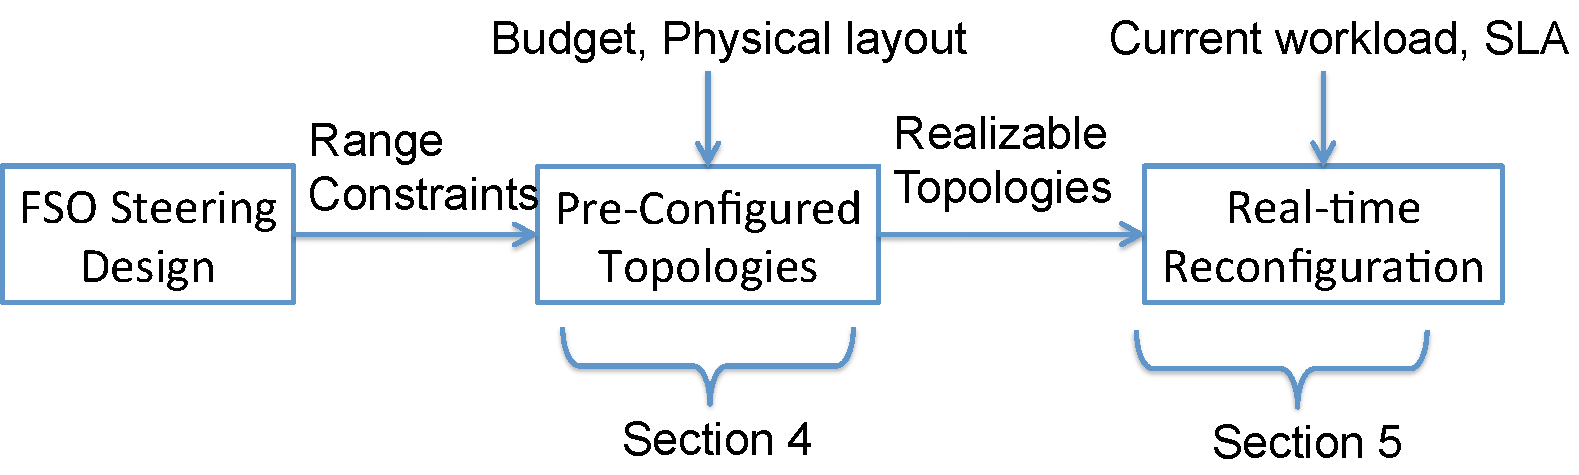
\includegraphics[width=220pt]{PPTFigs/OptimizationInteraction.pdf}
\caption{Interaction between the design constraints induced by FSO
steering choices, the selection of preconfigured topologies, and the
real-time topology selection} 
\label{fig:345}
\end{wrapfigure}

In our context, there are essentially two \blue{stages of network
  design} done at different timescales of operation.
\underline{First}, we need to {\em pre-configure} the network and FSO
assembly; e.g., choosing number of FSOs per rack, the specific
alignments of the different SMs, or \blue{scoping} the beam angle of
the GMs. This needs to be done at coarse time granularity (e.g.,
monthly), because of the time incurred in changing such a
pre-configuration setup. \underline{Second}, given this pre-configured
setup, we need to choose a {\em runtime} topology by activating a
subset of links, at finer timescales (i.e., few millseconds) based on
the prevailing traffic load. Thus, we envision the design workflow in
  Figure~\ref{fig:345}.  In this section, we focus on the first
  network design problem done at a coarser timescale, viz., the
  pre-configuration problem.  We defer the runtime operation (called
  {\em reconfiguration}) to Section~\ref{sec:reconfig}.

\green{Essentially, the pre-configuration problem is: Given an overall
  budget and phyiscal constraints, determine a range of network
  parameters---number of machines per rack, number of FSOs per rack,
  number of FSOs equipped with GM vs.\ SM, number of SMs per FSO, the
  pre-orientation of GMs, and the pre-alignment of SMs---that can
  deliver good performance.}
%
This problem is significantly different from prior theoretical work in
network design~\cite{} on two fronts: (1) {\em flexibility} requires
us to rethink topology design algorithms and traditional performance
metrics, and (2) the \ArchName hardware elements impose unique
physical, budget, and geometric constraints. Thus, we break down our
proposed research into two stages.  First, to \blue{understand the
  theoretical implications of topology flexibility}, we focus on a
more abstract problem of designing an optimal ``pre-configured
flexible topology'' (\PCFT). Then in Section~\ref{sec:bbo}, we use
these insights to revisit the budget-based \ArchName network design
problem.

\subsection{Foundations of Pre-Configured Flexible Topology Design (\PCFT)} 
\label{sec:pcft}

\begin{wrapfigure}{r}{160pt}
\vspace{-0.2in}
\centering
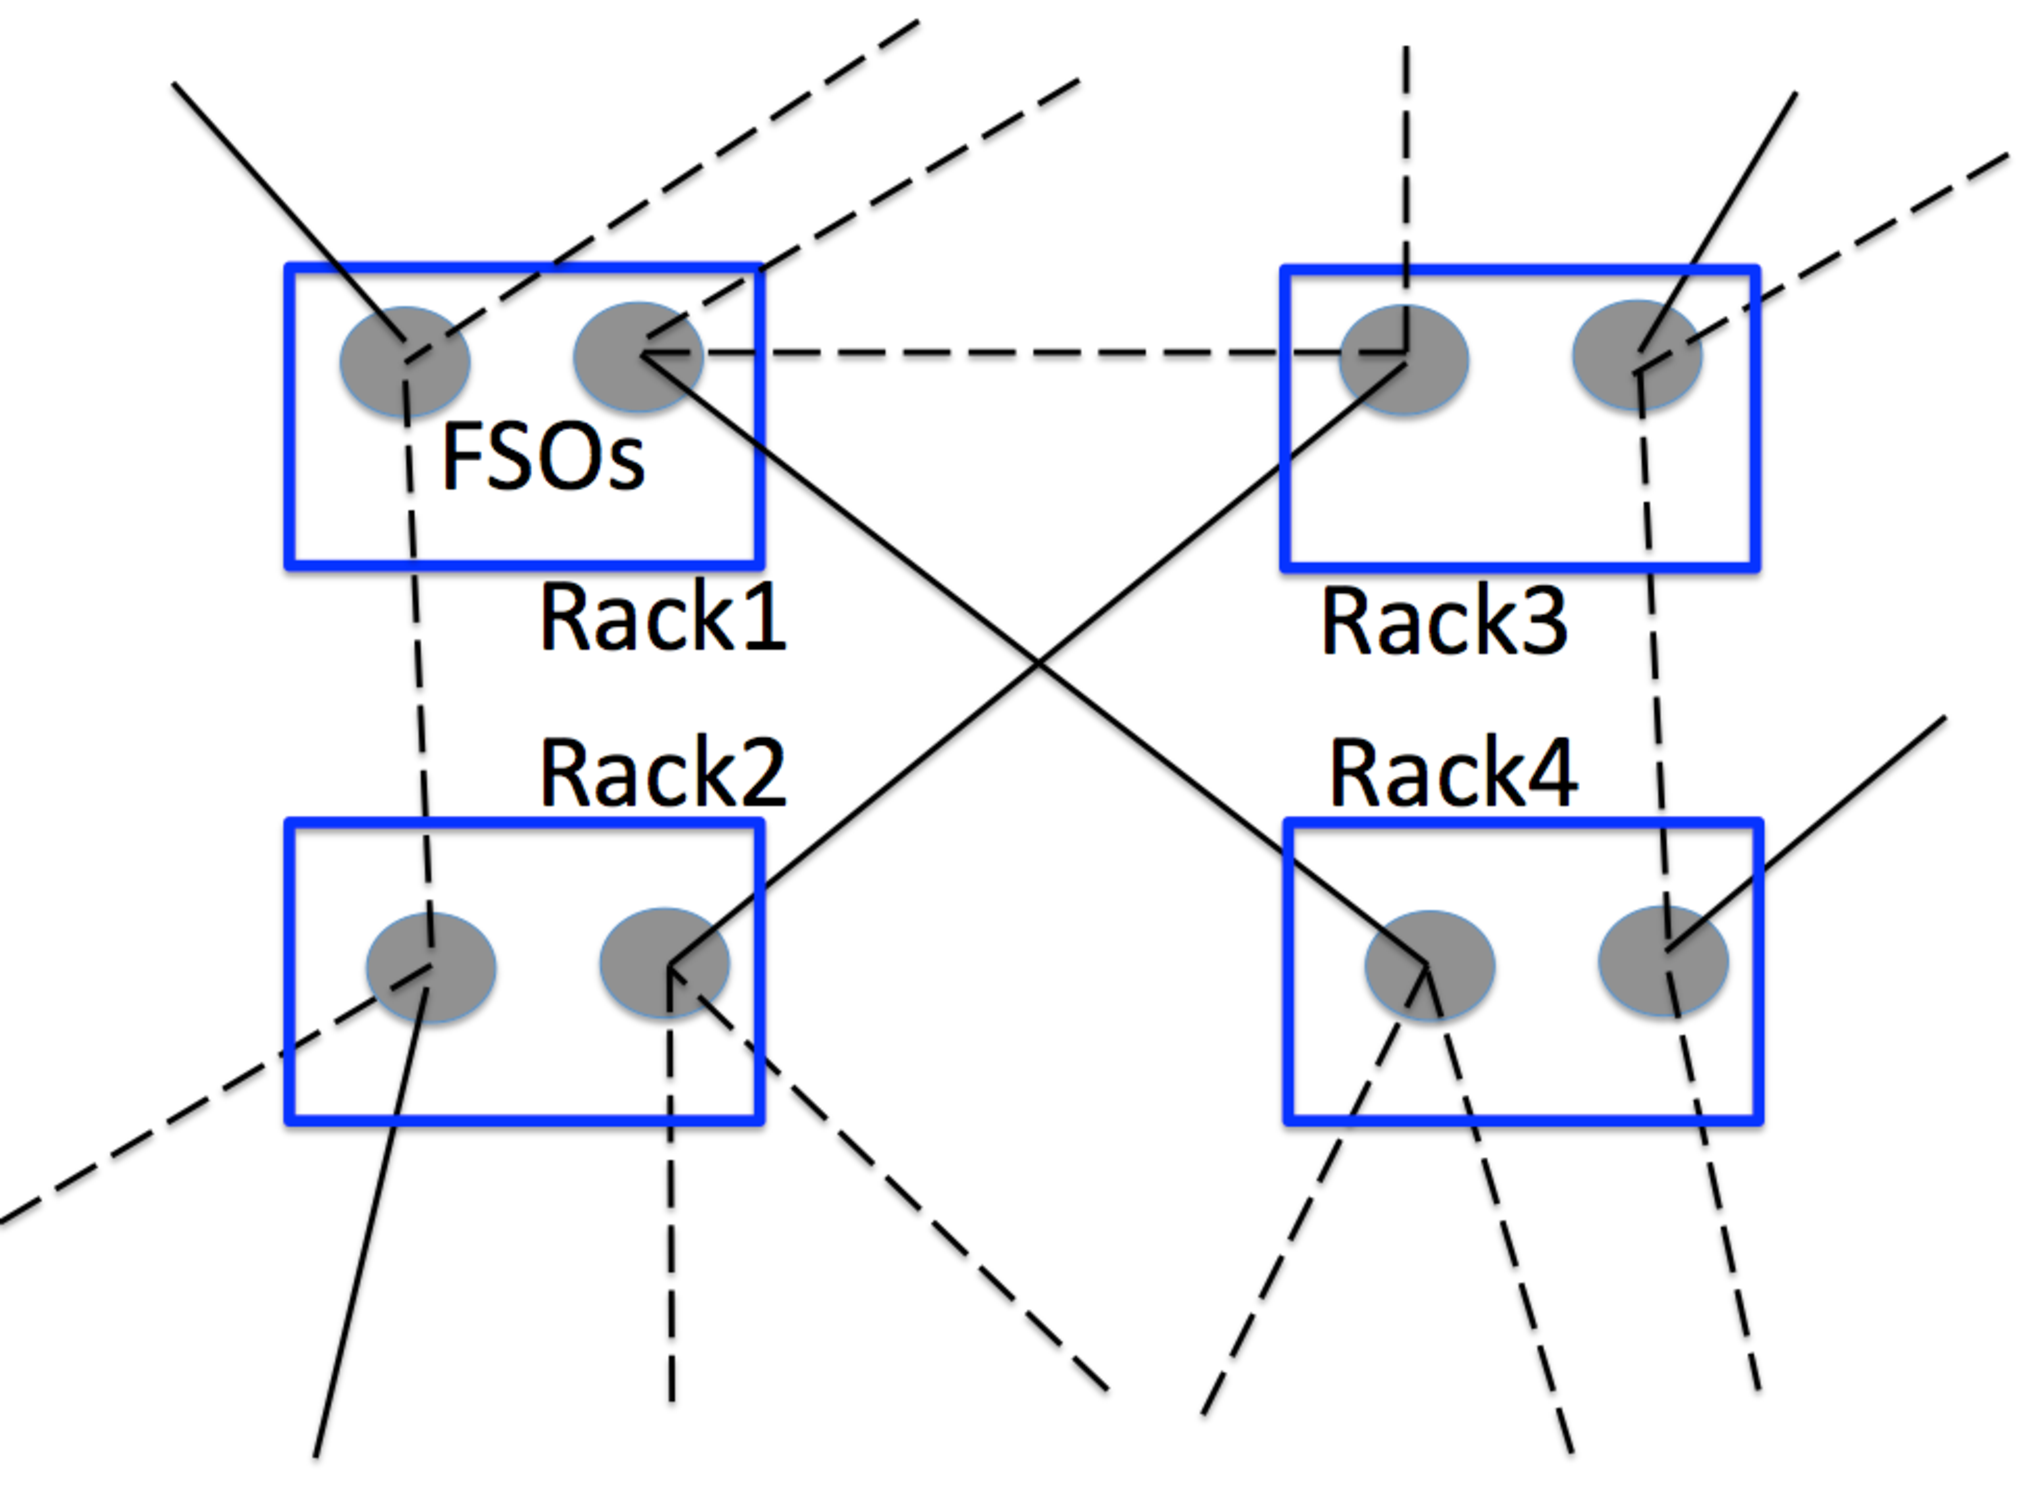
\includegraphics[width=160pt]{PPTFigs/pcft.pdf}
\vspace*{-0.4in}
\caption{A pre-configured flexible topology (PCTF) with candidate
  links (solid and dashed). Number of FSOs per rack ($m$) is 2, and
  the number of candidate links per FSO ($\FSODegree$) is 3. The set
  of solid (active) represents one possible realizable topology.}
\label{fig:pcft}
\end{wrapfigure}

To gain insights into the theoretical foundations of the problem, we
abstract away the details of the SM or GM or the cost budget and focus
on the following problem: Given the number of racks $\NumRacks$,
number of FSOs $\NumFSOs$ on each rack, and the maximum number of {\em
  candidate links} $\FSODegree$ per FSO \blue{that each FSO can be
  steered to}, the {\em pre-configured flexible topology (\PCFT)
  design problem} is to determine the set of links connecting pairs of
FSOs, so as to optimize the ``dynamic bisection bandwidth'' of the
network (defined below).

\softpara{Terminology.} A \PCFT essentially is a $k$-regular graph
over the $m$ FSOs, where each edge is called a {\em candidate link}
and represents an achievable communication link. However, at any point
during runtime, only one candidate link per FSO can be {\em active};
thus, the set of active links form a matching over the FSOs. Given a
\PCFT, any matching over the FSOs is called a {\em realizable
  topology} of the given \PCFT. See Figure~\ref{fig:pcft}.
%
\green{Thus, the PCFT problem can be thought of as constructing a
$\FSODegree$-regular graph over $\NumRacks\NumFSOs$-nodes such that
the {\em set} of matchings (i.e., realizable topologies) of the graph
maximizes the dynamic bisection bandwidth (defined next).}

\begin{task}
\label{task:pcft}
We will investigate the theoretical foundations of flexible topology
design that maximizes dynamic bisection bandwidth in conjunction with
other measures of network goodness (e.g., diameter).
\end{task}

\mypara{Rethinking Metrics for Flexible Topologies} The traditional
bisection bandwidth metric~\cite{} reflects a {\em static} perspective
of the topology. However, in our context, we should instead consider
the notion of {\em dynamic} bisection bandwidth (DBW) since different
realizable topologies can be used for different communication
requirements. Formally, the dynamic bisection bandwidth of a given
pre-configured topology $\Pi$ can be defined as follows. Let $T$ be
the set of realizable topologies of a given pre-configured topology
$\Pi$, $P$ be the set of partitions of the given network into two
equi-sized sets of machines, and $BW(t,p)$ be the bandwidth of a
(realizable or static) topology $t$ for the partition $p$ (i.e., the
cut-size in $t$ corresponding to $p$). Then, the traditional notion of
bisection bandwidth for a (static) topology $t$ is given by $\min_{p
  \in P} {\rm BW}(t, p).$, while the {\em dynamic bisection bandwidth}
DBW($\Pi$) for the pre-configured topology $\Pi$ is defined as:
$$\min_{p \in P} \max_{t \in T} {\rm BW}(t, p).$$

In addition to just maximizing DBW, we also consider the objective of
maximizing DBW under the constraint of bounded network diameter.
Network diameter is a reasonable way to bound worst-case latency,
which has also been considered as an objective in designing datacenter
topologies~\cite{rewire-20-39}. We also also use an appropriate notion
of {\em dynamic diameter} (as for DBW above) instead of the
traditional notion of network diameter.

\mypara{Connection to Known Graph Problems} In general, the PCFT
problem is in the class of the {\em network design problem
  (NDP)}~\cite{ndp-survey} (and more specifically, {\em
  degree-constrained subgraph} problem), wherein, given a graph, the
goal is to extract a (degree-constrained) subgraph satisfying some
design criteria and optimizing a given objective function.  What
distinguishes the PCFT problem from the prior-addressed NDP problems
is the choice of our objective function, viz., dynamic bisection
bandwidth.

The special case of the PCFT problem, when $\FSODegree=1$, actually
boils down to constructing an $\NumFSOs$-regular graph over
$\NumRacks$ nodes with maximum (static) bisection bandwidth. The
closest known problems to this $\FSODegree=1$ case of our PCFT problem
are: (a) Computing the bisection bandwidth of a given \blue{regular}
graph; this problem is known to be
NP-hard~\cite{bui-leighton-comb-1987}, with the best known
approximation-factor of $O((\log n)^2)$~\cite{fiege-focs-2000}. Our
PCFT problem is very different from this problem. (b) Determining an
upper-bound on the bisection bandwidth of $\NumFSOs$-regular graphs of
size $\NumRacks$, for a given $\NumFSOs$ and $\NumRacks$; this problem
has been addressed extensively, and non-tight upper-bounds (have been
determined for small values (upto 4) of
$\NumFSOs$~\cite{monien-2006}. Note that this upper-bound problem can
actually be reduced to the $\FSODegree=1$ version of our PCFT
problem. {\it The above results suggest that the PCFT problem is very
  likely intractable, even for $\FSODegree=1$.}


\mypara{Proposed Approaches} We will pursue three different approaches
for the PCFT problem. The first approach builds upon designs with high
static bisection bandwidth, the second approach builds upon solutions
to special cases of the dual-problem, while the third is a heuristic-based
approach.

\begin{packeditemize}
\item {\em Static to Dynamic Conversion.} One reasonable approach to
  solve the PCFT problem would be to start with constructing a
  $\NumFSOs\FSODegree$-regular graph of $\NumRacks$ nodes with a high
  (static) bisection bandwidth, and then group the
  $\NumFSOs\FSODegree$ candidate links at each node into $\NumFSOs$
  sets of $\FSODegree$ links each so as to maximize the dynamic
  bisection bandwidth. For the \underline{first step}, there are only
  a few results on explicit construction of general graph classes with
  high bisection bandwidth~\cite{peres}. In particular, $d$-regular
  Ramanujan Graphs~\cite{rewire-18} of are known to have a bisection
  width of at least $((d/2 - \sqrt(d-1))n/2$, but their construction
  is mostly algebraic. Other graph classes of interest are Cage
  graphs~\cite{cage}, which have a large \blue{girth} (length of
  smallest cycle). In our specific context of small values (a few
  hundreds) of $\FSODegree\NumFSOs$ and $\NumRacks$, we can
  investigate bisection bandwidth of certain classes of regular
  graphs, and pick ones that suggest a high bisection bandwidth
  \blue{with low diameter}; in particular, due to symmetry of
  nodes/racks, we can also restrict ourselves to ``symmetric'' regular
  graph such as distance-transitive graphs. For the \underline{second
    step} of grouping candidate links, we will employ certain
  heuristics. E.g., we can number the $\NumRacks$ nodes from 1 to
  $\NumRacks$ and group the $\NumFSOs\FSODegree$ links into $\NumFSOs$
  sets based on the ranges of node numbers they connect to. Such a
  heuristic will guarantee a ``uniform'' division of links into sets
  across the nodes.

\item {\em Dual-based Approach.}  If each rack contains
  $\NumMachinesPerRack$ machines and the links (between a machine and
  the ToR switch, or a pair of FSOs) have a unit bandwidth, then the
  optimal desired bisection bandwidth is
  $\NumRacks\NumMachinesPerRack/2$. We note that, for uniform link
  bandwidths, the inter-rack and inter-machine bisection bandwidths
  are same. Now, let us consider what values of $\FSODegree$ and
  $\NumFSOs$ can enable this DBW value of
  $\NumRacks\NumMachinesPerRack/2$. We consider two extremes: (a) If
  $\FSODegree=1$, then it can be shown that \blue{$\NumFSOs =
    \min(\NumRacks/2+\NumMachinesPerRack, 7\NumMachinesPerRack)$
    suffices\footnote{By using $7l$ ports on a ToR switch, we can
      simulate a Fat tree architecture.} (but not necessarily
    optimal).} For large values of $\NumRacks$ and
  $\NumMachinesPerRack$, it is known~\cite{book-28-29} that
  $\NumFSOs=2\NumMachinesPerRack$ would almost always work. (b) If
  $\FSODegree$ can be an arbitrarily high, then the optimal value of
  $\NumFSOs$ required is $\NumMachinesPerRack$ (for $\FSODegree=n/2$);
  here, for $\NumFSOs=l$, the $\FSODegree$ required (=$\NumRacks/2$)
  is also optimal. The above resuls hold for any DBW value that is an
  integral multiple of $\NumRacks$.
%
The above near-optimal solutions for certain special cases of the
``dual'' problems (i.e., given a desired DBW value, minimize $\NumFSOs$ or
$\FSODegree$ for a given $\NumRacks$ value) gives us some insights into solving the
PCFT and its dual problems.  In particular, if we can solve the above
dual problem of minimizing $\NumFSOs$, given $\FSODegree$, $\NumRacks$, and a desired DBW
value, for arbitrary $\FSODegree$ values and integral of $\NumRacks$ values of DBW,
then it is easy to derive an approximation algorithm for the PCFT
problem that has only an {\em additive} approximation-factor of $\NumRacks$.

\item{\em Simulated Annealing (SA-PCFT).}  Simulated Annealing (SA)
  heuristics~\cite{} have been used with great success for
  optimization problems. \blue{In our context, since the PCFT design
    is done offline, we can afford the convergence time incurred by an
    SA approach.}  To design an SA approach for our PCFT problem, we
  need three key components: \underline{First}, we need good ``seed''
  (starting) solutions; here, we could use one of our earlier
  approaches, or as in~\cite{rewire}, use graphs with a ``large
  spectral gap''~\cite{rewire,spectral,rewire-18} which are known to
  have desirable properties (e.g., low
  diameter~\cite{spectral-diameter}).  \underline{Second}, we need
  ways to generate ``neighboring'' solutions; for this, we can use
  \blue{simple transformations} that transform a regular graph to
  another. E.g., the transformation that changes the edges ${(a,b),
    (c,d)}$ to ${(a,c), (b,d)}$ can be used iteratively to construct
  any regular graph from another.  \underline{Lastly}, we need an
  efficient heuristic for computing DBW (PCTF's objective function) of
  a given graph; for this, we will investigate generalization of the
  following approaches: (i) Well-known efficient heuristics, viz.,
  SA~\cite{} and Kernighan-Lin~\cite{} for computing the bisection
  bandwidth, and (ii) a recent result~\cite{rewire} that uses Valiant
  (or, two-state) load balancing technique~\cite{valiant} to compute a
  {\em lower bound} on the bisection bandwidth.

  The above SA-PCFT approach can also be generalize to maximize an
  appropriately defined {\bf traffic-aware DBW objective}, based on
  coarse statistics available on inter-rack traffic. \green{Note that
    since pre-configuration can only be done on an infrequent basis
    (e.g., weekly), so we are only interested in coarse traffic
    knowledge.}  One simple form of inter-rack traffic statisfics
  could be in the form of a weights between every pair the racks, and
  the DBW definition can be appropriately tailored as
  in~\cite{leighton-99} for multi-commodity min-cut. \blue{In our
    research, we will also consider incoporating more sophisticated
    traffic models~\cite{}.}
\end{packeditemize}

\subsection{Budget-Based Optimization}
\label{sec:bbo}

Formally, given the total number of machines to interconnect, physical
constraints, overall budget, and pricing of relevant hardware devices,
the \BBO problem is to determine the following such that the dynamic
bisection bandwith is maximized: (a) Number of machines
($\NumMachinesPerRack$) per rack and thus, the number of racks
($\NumRacks$), (b) number of FSOs ($\NumFSOs$) per rack and thus, the
number of ports on the ToR switch, (b) Number of FSOs ($\NumFSOsWithGM
\leq \NumFSOs$) that are each equipped with a GM and the number of SMs
($\NumSMsPerFSO$) on each of the remaining $(\NumFSOs -
\NumFSOsWithGM)$ FSOs, on each rack, and (c) the {\em pre-orientation}
of each of the GMs and {\em pre-alignment} of each of the SMs in the
system.

\begin{task}
\label{task:bbo}
We will design efficient algorithms for the Budget-Based Optimization
Problem (\BBO) with the objective of maximizing dynamic bisection bandwidth.
\end{task}

\mypara{Proposed Approach} Based on our insights from the previous
section, we will use the following approaches to address the \BBO
problem:

\begin{packeditemize}
\item
{\em PCFT-Based Algorithm.}  We can use any of the PCFT algorithms as
a subroutine to solve the BBO problem as follows. \underline{First},
we convert the given budget and physical constraints, and the pricing
information into a constraint equation over $\NumRacks$ (number of
racks), $\NumFSOs$ (number of FSOs per rack), and $\FSODegree$ (the
number of candidate links per FSO). \blue{To constrain $\FSODegree$,
  note that $\FSODegree\NumFSOs = c\NumFSOsWithGM + (\NumFSOs -
  \NumFSOsWithGM)\NumSMsPerFSO$, where $c$ is the number of candidate
  links a GM can be steered to use and can be assume to be a
  constant.}
%
\underline{Second}, we solve the PCFT problem for various $\NumRacks$,
$\NumFSOs$ and $\FSODegree$ that satisfy the above budget constraint
for a given $\NumFSOsWithGM~(\leq \NumFSOs$).  Then, we convert each
PCFT solution to a design realizable by $\NumFSOsWithGM$ GMs and
($\NumFSOs - \NumFSOsWithGM$) sets of $\NumSMsPerFSO$ SMs each, on
each rack, and estimate its DBW using one of the approaches described
earlier. \underline{Lastly}, we explore the space of
$\NumRacks,\NumFSOs,\FSODegree, \NumFSOsWithGM$ efficiently using
standard search techniques, to compute an efficient network design for
the given budget and pricing.

\item
{\em Extending SA-PCFT.}  We can modify our Simulated Annealing
approach for the PCFT problem to solve the \BBO problem, by
appropriately modifying the transformation operator to generate
neighbors of a particular network design. Here, the neighbors of a
design may include designs with slightly different values of
parameters $\NumRacks$, $\NumFSOs$, $\FSODegree$, $\NumFSOsWithGM$,
and/or candidate links, under the budget constraints.
\end{packeditemize}
